%========================================================================================
% TU Dortmund, Informatik Lehrstuhl VII
%========================================================================================

\chapter{Spring-Algorithmus}
\label{Kapitel 2}
%
In diesem Kapitel werden die Grundlagen des Spring-Algorithmus erklärt. 
Es geht um die Verwendung dieser Algorithmen, das grundsätzliche Vorgehen
und die Erweiterbarkeit.



\section{Spring-Algorithmus - Einleitung und Verwendung}
\label{Kapitel_2_-_Unterkapitel_1}
%
Das Problem der Darstellung eines Graphen existiert schon sehr
lange. Es basiert auf der Platzierung der Kanten sowie
Knoten um eine möglichst ästhetische Zeichnung des
Graphen zu erhalten, die gut lesbar und verständlich ist. ([3] Seite 2-3 )
Um dies zu erreichen gibt es verschiedenste Ansätze. Im 
Folgenden wird es um ein Verfahren gehen, welches auf ein Modell
der Physik zurückgreift. 

Verschiedenste Partikel ziehen sich an oder stoßen sich ab. Man 
kann sich diese anziehende und abstoßende Kraft als eine Feder
vorstellen. Existiert eine anziehende Kraft zwischen den Partikel so
ist diese Feder gespannt, bei einer abstoßenden Kraft belastet. 
Nimmt man sich diese Modell zugrunde, so stehen die Partikel
für Knoten und die Federn für Kanten. Diese richten 
sich anhand ihrer Kraft solange aus, bis keine weitere Energie 
mehr im System ist. ([4] Seite 1130 ff.) Das führt zu einer ästhetischen
Zeichnung des Graphen. In der Abbildung 2.1 wird dieser Prozess einmal
dargestellt.

    \begin{figure}[t]
    	\centering
    	{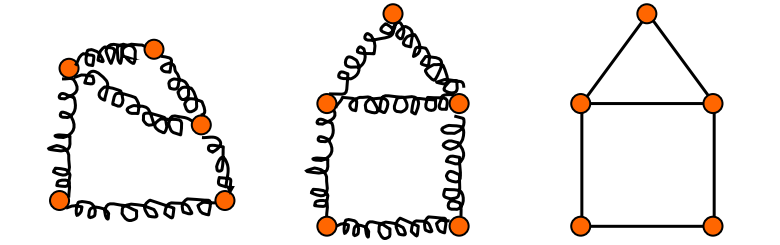
\includegraphics[scale=0.8]{bilder/graphfeder}\label{fig_graphfeder}
    	}\\
    	\caption[Darstellung der Kanten als Federn]{Darstellung der Kanten als Federn}
    	\label{fig_testbild2}
    \end{figure}



\section{Spring-Algorithmus - Pseudocode}
\label{Kapitel_2_-_Unterkapitel_2}
%

Zwischen jedem Knotenpaar wird eine abstoßende Kraft \begin{math} f\textsubscript r \end{math} berechnet. Alle
benachbarten Knoten erhalten eine anziehende Kraft \begin{math} f\textsubscript a \end{math}. Zwei Knoten \begin{math} u,v \in V \end{math}sind benachbart wenn \begin{math} uv \in E \end{math} ist. Das führt dazu, dass verbundene Knoten näher zusammen
gezeichnet werden, während sie noch immer einen gewissen Abstand zueinander
haben. Der Algorithmus geht dabei in drei Schritten vor:

\begin{enumerate}
	\item zwischen jedem Knotenpaar die abstoßende Kraft berechnen
	\item benachbarten Knoten eine anziehende Kraft zuweisen
	\item jeden Knoten seiner neuen Kraft nach bewegen
\end{enumerate} 
Diese drei Schritte werden werden so oft wiederholt bis das System keine
übrige Energie mehr hat und sich kein Knoten mehr bewegt.

    \begin{algorithm}[t]
    	\centering
    	\caption[Ein Algorithmus]{Fruchterman und Reingolds Algorithmus} \label{algo_1}
    	\begin{algorithmic}
    		\REQUIRE \begin{math} G:= (V,E) \end{math}
    		\ENSURE \begin{math} G:= (V,E) \end{math} mit besserer Positionierung
    		\FOR{\begin{math}i:=1 \leq iterations \end{math}}
    		\FOR{\begin{math}v \end{math} \textbf{in} \begin{math}V\end{math}}
    		\STATE $v.disp := 0;$
    		\FOR{(\begin{math}u \end{math} \textbf{in} \begin{math}V\end{math})}
    		\IF{$u\neq v$}
    		\STATE $\Delta := v.pos - u.pos;$
    		\STATE $v.disp := v.disp + (\Delta / |\Delta|) * f\textsubscript{r}(|\Delta|));$
    		\ENDIF
    		\ENDFOR
    		\ENDFOR
    		\newline
    		\FOR{\begin{math}e \end{math} \textbf{in} \begin{math}E\end{math}}
    		\STATE $\Delta := e.v.pos - e.u.pos;$
    		\STATE $e.v.disp := e.v.disp - (\Delta / |\Delta|) * f\textsubscript{a}(|\Delta|));$
    		\STATE $e.u.disp := e.u.disp + (\Delta / |\Delta|) * f\textsubscript{a}(|\Delta|));$
    		\ENDFOR
    		\newline
    		\FOR{\begin{math}v \end{math} \textbf{in} \begin{math}V\end{math}}
    		\STATE $v.pos := v.pos + ( v. disp/ |v.disp|) * min ( v.disp, t );$
    		\STATE $v.pos.x := min(W/2, max(-W/2, v.pos.x));$
    		\STATE $v.pos.y := min(L/2, max(–L/2, v.pos.y))$
    		\ENDFOR
    		\ENDFOR
    	\end{algorithmic}
    \end{algorithm}

Fruchterman und Reingold haben ihre Funktionen \begin{math} f\textsubscript r \end{math} und \begin{math} f\textsubscript a \end{math} aus ihrer Arbeit 1984 wie folgt definiert:

   
	\begin{align*}
		f\textsubscript a (d) =
			d^{2}/k
	\end{align*}
    
    \begin{align}
		f\textsubscript r (d) =
		-k^{2}/d
    \end{align}

während \begin{math} k \end{math} für die optimale Distanz zweier Knoten steht:

    \begin{align}
    	k =
    	\sqrt{Area / |V|}
    \end{align}

\begin{math} Area \end{math} ist die zur Verfügung stehende Fläche:

    \begin{align}
    Area =
    W * L
    \end{align}
  
\section{Spring-Algorithmus - Erweiterbarkeit}
\label{Kapitel_2_-_Unterkapitel_3}   
Eine besondere Eigenschaft dieses Algorithmus ist die leichte Erweiterbarkeit. Er kann leicht an viele verschiedene Probleme angepasst werden.
Der Algorithmus 2.1 ist bereits eine erste Erweiterung des ursprünglichen Algorithmus. Beim Bewegen der Knoten im dritten Schritt wird sichergestellt, dass sich die Knoten weiterhin auf der zur Verfügung stehenden Fläche befinden.


%
